%%%%%%%%%%%%%%%%%%%%%%%%%%%%%%%%%%%%%%%%%%%%%%%%%%%%%%%%%%%%%%%%%%%%%%%%%%%%%%%%%%
%% For technical support please email: ykoh@wspc.com.sg (or) rajesh@wspc.com.sg %%
%% The content, structure, format and layout of this style file is the          %%
%% property of World Scientific Publishing Co. Pte. Ltd.                        %%
%% Copyright 2014 by World Scientific Publishing Co.                            %%
%% All rights are reserved.                                                     %%
%%                                                                              %%
%% Proceedings Trim Size: 9in x 6in                                             %%
%% Text Area: 7.35in (include runningheads) x 4.5in                             %%
%% Main Text is 10/13pt                                                         %%
%% Last Modified: 24-01-2014                                                    %%
%%%%%%%%%%%%%%%%%%%%%%%%%%%%%%%%%%%%%%%%%%%%%%%%%%%%%%%%%%%%%%%%%%%%%%%%%%%%%%%%%%
%
%\documentclass[wsdraft]{ws-procs9x6}  % to draw border line around text area
%\documentclass[wssquare]{ws-procs9x6} % for citations in square brackets (consult your editor before picking up this style)
\documentclass{ws-procs9x6}            % default, citations in superscript
\usepackage{lmodern}

\begin{document}

\title{Recommender systems with heterogeneous information network for cold start items}

\author{Di Zhang, Qian Zhang, Guanquan Zhang, Jie Lu}

\address{\textit{Decision Systems and e-Service Intelligence Laboratory,} \\
\textit{Centre for Artificial Intelligence}\\
University of Technology Sydney, Australia \\
Di.Zhang-7@student.uts.edu.au, Qian.Zhang-1@uts.edu.au \\
Guangquan.Zhang@uts.edu.au, Jie.Lu@uts.edu.au}

\begin{abstract}
Recommender System has been widely adopted in real-world applications. Collaborative Filtering (CF) and matrix based approach has been the forefront for the past decade in both implicit and explicit recommendation tasks. One prominent challenge most recommendation approach facing is dealing with different data quality conditions. i.e. cold start and data sparsity. Some model based CF methods use condensed latent space to overcome sparsity problem. However, when dealing with constant cold start problem, CF approach can be ineffective and costly. In this paper, we propose MERec, a novel approach that adopts graph meta-path embedding to learn item/user features independently besides learning from user-item interactions. Such approach allows unseen data to be incorporated as part of user/item learning process, hence effectively reduce the impact in cold start problem for new or sparse dataset.
\end{abstract}

\keywords{recommender system; cold-start; heterogeneous information network.}

\bodymatter

%!TEX root = ./main.tex
\section{Introduction}

Recommender system is an indispensable technology in this big data era \cite{lu2015recommender}. It help us to find personalized products or services from the ever-increasing information overloads and make our life more efficient and focused. Collaborative Filtering (CF) and matrix based approach are a dominant recommendation approach For the past decades. Most of the works require user-item interactions to be presented for training. Consequently, a warming up period is commonly required for CF based approach to over come the data sparsity problems, due to continuously evolving data.

Traditionally, matrix factorization approach projects user/item features into a latent space. then calculate user-item similarity based on their condensed latent vector values. However, such methods are not suited in dealing brand new items, which have a profound use case in real-world scenarios. A known workaround is running a routine end to end re-train process to pick up new interactions, which can be inefficient and costly. Content or hybrid approach, are one way to over come the problem. It is proven to be challenging when dealing large categorical features, such as exponential computation complexity increase, as well as introducing noise.

Recently, many embedding method is developed via HIN based approach \cite{mao2016multirelational,wang2016member}. Graph data structure enables continuously adding user/item feature related information. The embedding process item/users' representation can be learned based on nodes' local and global structure, via process such as random walk. For example, Node2vec, DeepWalk \cite{grover2016node2vec} \cite{perozzi2014deepwalk}. However, Random walks based presentation learning are known to be more biased to highly connected nodes. \cite{sun2011pathsim}. Meta-Path based approach \cite{dong2017metapath2vec} helps in controlling random walk probability for improved embedding result. Though, there are a number of research shown promising results in explicit recommendations problem. The cold start problem is little discussed, especially with the implicit recommendation domain. Problems, such as, optimizing click through rate without ratings have much wider real-world applications, and severer cold problem. 

In this paper we propose a Meta-path Embedding based Recommendation (MERec), a novel approach that utilizing meta-path based presentation learning on HIN. This approach is primarily focusing on solving the cold start problems when data is continuously evolving. The model is also designed to be adaptive to newly emerged data, so that recommendation could be made even there is zero user-items interaction available. By translating domain experts relevancy rules into meta-path set, our approach allow a controlled random walk to reduce computation intensity and improve on end result. 

We Identify the paper contributions as following:
\begin{itemize}
    \item a novel fusion approach to effectively handle fresh data problem in implicit recommendation problem;
    \item a controlled approach that capable in incorporating expert knowledge into training process;
    \item a framework that can effectively reduce end to end retraining interval when data keep evolving overtime;
\end{itemize}

The rest of this paper is constructed as follows: In Section II, we discuss the related research and relevant definition that helped our research. In Section III, we explain our framework and related algorithms. In Section IV, we show our experiment design and result comparison with other models in different cold and non-cold start scenario. Lastly In Section V, we discuss our finding and and explore future improve directions.

%!TEX root = ./main.tex
% \section{Related Works}
% Graph based presentation learning is a actively researched topic in areas such as node classification, clustering, and similarity search. As intuitively, objects similarity can be measured based on node distance and density of given graph/sub-graph. Studies such as P-PageRank \cite{bahmani2010fast}, SimRank \cite{jeh2002simrank}, leverage homogeneous network structures. While research like PathSim \cite{sun2011pathsim}, HeteSim \cite{shi2014hetesim} manages to taking different types of objects and links in to data mining process, so that different semantic meaning across different types of nodes can be learned respectively. With the advancement of NLP research, i.e. Word2Vec \cite{mikolov2013efficient}. Embedding methods are introduced into node presentation learning. For example, node2vec \cite{grover2016node2vec} adopts CBOW and SkipGram into random walk process. Subsequently, Metapath2Vec \cite{dong2017metapath2vec} introduced a guided random walk approach to help reduce the bias of random walk, by introducing a set of predefined meta-path. 

% Since `The Netflix Prize' \cite{bennett2007netflix}. Memory based CF measures similarity by using Pearson Correlation or vector cosine similarities to derive predictions though a aggregated nearest neighbor mechanism. Model based CF leverage data mining techniques by learning user/item latent features. As knowledge graph and especially Graph Neural Networks gaining traction \cite{wu2019comprehensive}, there are a number of HIN based techniques being developed such as item2vec \cite{Barkan2016}, entity2vec \cite{palumbo2017entity2rec}. and HErec \cite{shi2018heterogeneous} towards user-item ratings predictions. Though, We are not able to see much research results on the implicit recommendation front. 

% Hence, we propose MERec, a framework that is motivated on solving cold start problems on implicit predictions using HIN. 

\section{Preliminaries}\label{3PD}
Following definitions are used for describe our approach.

\begin{definition}[Heterogeneous Information Graph]
An information graph is $G = (V,E)$, where $V$ is the set of nodes (or entities) of the graph. $E$ is the set of edges connecting the nodes in $V$, $E \subset V \times V$.

Two mapping functions: Entity type mapping function $\phi$: $V \rightarrow A$, and link type mapping function $\varphi$: $E \rightarrow R$, where $A$ and $R$ denote the sets of predefined entity and link types, and $|A| > 1$ or $|R| > 1$ indicating that there are more than one type.
\end{definition}

Graph schema indicates how different types of entities link with each other. It serves as a template to describe the structure as well as the semantic relationship between object types.
\begin{definition}[Meta-Path]\label{def:metaPath}
A Meta-Path $\mathcal{P}$ is a path defined on the  graph schema $T_G = (A, R)$. \newline
Meta-Path $\mathcal{P}$ is denoted as $A_1 \xrightarrow{\text{r1}} A_2 \xrightarrow{\text{r2}} \dots \xrightarrow{\text{rn}} A_n$. 

Relationship $R$ is denoted as $r1 \bullet r2 \bullet ... rn$ for different types of relationship between different types of entity nodes, where $\bullet $ denotes composition operator or relations.
\end{definition}

For Meta-Path $\mathcal{P}_i$ shares same graph schema, there could also be multiple path $p$ connecting source entity $a_i$ to target ${a}_{i+1}$. Each path $p$ inside Meta-Path $\mathcal{P}_i$ is a path instance, $p \in \mathcal{P}_i$. The number of path instances $p$ between $a_i$ and $\bm{a}_\text{i+1}$, is called path count. Reverse Meta-Path $\mathcal{P}^{'}$ is the reversed relation sequence of $\mathcal{P}_i$, if $\mathcal{P}^{'}$ is the reverse path of $\mathcal{P}$ in $T_G = (A, R)$, reverse path is denoted as $\mathcal{P}^\text{-1}$. \newline

Meta-Path $\mathcal{P}_1: A_1 \xrightarrow{r_1} A_2$ is the Meta-Path connects source entity type $A_1$ and target $A_2$.
Similarly, $\mathcal{P}_2: A_2 \xrightarrow{r_2} A_3$, $\mathcal{P}_2$ is the Meta-Path between source entity type $A_\text{2}$ and target entity type $A_\text{3}$.
Here we call $\mathcal{P}_1$ and $\mathcal{P}_2$ are contactable. Then $\mathcal{P}_1$ and $\mathcal{P}_2$ can be combined as $\mathcal{P}_{1,2}: A_1 \xrightarrow{r_1} A_2 \xrightarrow{r_2} A_3$. For example, $Movie \rightarrow Director$ and $Director \rightarrow Movie$ can be combined to $Movie \rightarrow Director \leftarrow Movie$. 


%!TEX root = ./main.tex
\section{Meta-Path Embedding based Recommendation}

\begin{figure*}[!t]
    \centering
    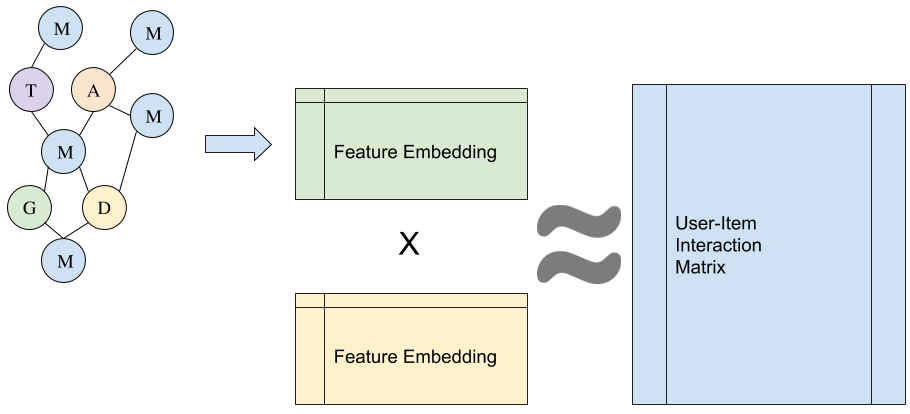
\includegraphics[width=0.8\textwidth]{figs/fig0.png}
    \caption{workflow of MERec}\label{fig:fe-overview}
\end{figure*}

In this Section, we propose MERec that meta-path based embedding and Bayesian Probability Ranking to overcome cold start problem. 

The key idea of our approach is inspired by recent research on graph-based embedding \cite{dong2017metapath2vec}. Unlike traditional matrix based approach, which learns user/item latent representation jointly based on user-item interactions matrix.\cite{rendle2012bpr} Our one breaks down item and user latent matrix learning through 2 separate steps. as illustrated in Fig. \ref{fig:fe-overview}. Item embedding is first learned based on item and its features nodes within HIN with a user defined meta-path sets for the moderating its random walk process. Then user latent feature is trained though Factorization Machine, which is optimized by using Bayesian Probability Ranking.

\subsection{Step 1: Item Embedding via Meta-path Based Random Walk}\label{3MF}

For items such as movies, books, music, there are a number of factors impacting users' decision. Instead of taking the one-hot encoding approach for category value. We first propose to treat different categorical information as separate node types. 
By leveraging domain knowledge we can form a heterogeneous information graph and sets of user defined meta-path for item-item similarities learning. 

For example, movie choice is closely linked to directors and its casts. Thus $Movie \rightarrow Director \leftarrow Movie$, $Movie \rightarrow Actor/Actress \leftarrow Movie$  can be very important meta-path in deciding how similar 2 movies are. We use those insights as a guideline to define meta-path from a heterogeneous information graph for item features embedding. As shown in Fig. \ref{fig:fe-graph}.
Each meta-path can derive a item-item similarity matrix $\mathbb{R}_i(\mathcal{P}_i)$, each different meta-path can be regarded as bias toward different feature aspects, so items co-occurrence can be learned separately under different meta-path.

\begin{figure*}[!t]
    \centering
    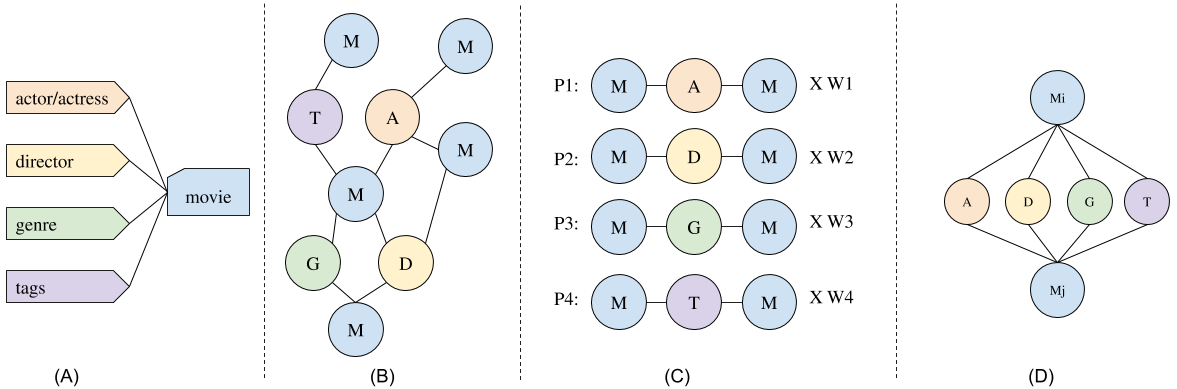
\includegraphics[width=0.8\textwidth]{figs/fig1.png}
    \caption{heterogeneous information graph based on item features}\label{fig:fe-graph}
\end{figure*}

as a result, item-item similarity score can be calculated by normalized meta-path similarity times meta-path weight.
\begin{equation}\label{itemsim}
    \mathcal{S}(v_i,v_j) = 
    \begin{cases}
         \sum\limits_{\substack{n=1}}^{n} \mathcal{R}_ij(\mathcal{P}_n,{W_n}),& \text{if } (v_{i}, .., v_{j}) \in \mathcal{P} \\
         0,              & \text{otherwise}
     \end{cases}
\end{equation}

$\mathcal{S}(v_i,v_j)$ stands for similarity between items $v_i$ and $v_j$ which shares the same node type. $R_ij()$ is a similarity function, where $\mathcal{P}_n, {W_n}$ stands for individual meta-path and its weights respectively. This end result provides guidance for the random walkers on our heterogeneous graph of item features. $(v_{i}, .., v_{j})$ is denoted as a meta-path instance, where $v_i$ is the starting node and $v_j$ the end node.

Given a heterogeneous graph $G = (V,E)$, and a meta-path set $[\mathcal{P}_1, \mathcal{P}_2, ... \mathcal{P}_n]$, the probability of transition is defined as following:
\begin{equation}\label{hetewalker}
    P(v_{i+1},\mathcal{P},w)= 
        \begin{cases}
            p({N^{t+1}(v_{i}^t)}),& \text{if } (v_{i+1}, .., v_{i}^t) \in \mathcal{P} \\
            0,              & \text{otherwise}
        \end{cases}
\end{equation}
where $t$ is denoted as $t^th$ steps, as the walker traversing through the graph and $p({N^{t+1}(v_{i}^t)})$ is a $softmax$ function on top of the neighbors of node $v_{i}^t$ as $p({N^{t+1}(v_{i}^t)}) = \frac{Exp(\mathcal{S}(v_i,v_j))}{\sum\limits_{\substack{n=1}}^{n} {Exp(\mathcal{S}(v_i,v_j)})}$.

We enable skip-gram \cite{mikolov2013distributed} to learn the presentation of given node $v$:
\begin{equation}\label{skipgram}
    arg max
    \sum\limits_{\substack{v \in V}}
    \sum\limits_{\substack{c \in N(v)}}
    \log p({c|v;\theta})
\end{equation}
where$\log p({c|v;\theta}))$ is defined as above. $c$ is denoted as $context$, in graph structure setting, $c$ is the neighboring nodes of given node $v$, i.e. $N(v)$. 

During the item embedding learning, we introduce 3 hyper parameters to learn the item vector representation. $d$ for dimension size, $x$ for number of walks, and $l$ for depth of each random walk.

By the end of this step, what we have is the item representation being projected in to a latent embedding space with reduced the complexity and sparsity issue comparing to content based approach. In Section \ref{4_experiment}, we will show more detailed comparison with categorical one-hot encoding.

\subsection{Step 2: User Latent Feature Learning}\label{3PCC}
After having feature embedding learned. Instead of learning $U, V$ jointly, we replace $V$ with the meta-path based item embedding vectors $Vec(v)$. This approach provides several benefits:

\begin{enumerate}
    \item Reducing learning complexities.
    \item Taking both item features and user-item interactions into account.
    \item $Vec(v)$ is not impacted even though user-item interactions are sparse.
\end{enumerate}

We use Bayesian Probability Ranking as our optimization objective:

\begin{equation}
    arg max
    \sum\limits_{\substack{v \in V}}
    (u_i \cdot Vec(v)-u_j \cdot Vec(v)) - \dfrac{\lambda}{2}tr(U^TU)
\end{equation}

Where $u_i \cdot Vec(v)$ is a positive interaction between item $v$ and user $i$, while $u_j$ is a randomly selected negative sample.
A fixed item embedding, also means during the training process user matrix is trained to fit the user-item interaction based on the item embedding. 
This means users representation is optimized independently based on item-feature embedding. As a result, the end user-item similarly score are equally effective for both observed and user-item pairs and brand new items. This characteristic ensures the final result to be effective on data sparsity problem as well as pure cold start problem.

Finally, we rank user candidate based on a dot product between trained user vector and item embedding vector. $ score = u \cdot Vec(v)$



% Based on the experiment result in Section \ref{4_experiment}, we see MERec out performs widely used CF+BPR by a large margin. It also gained equivalent or minor advantage when the dataset is less sparse in non-cold start settings.

%!TEX root = ./main.tex
\section{Experiments and Results}\label{4_experiment}
We have run a number of experiments based on several common real world scenarios, and we compared our approach with other popular methods through the experiments.
% \begin{itemize}
%     \item How effective MERec performs in $Pure$ $Cold$ and $Sparse dataset$.
%     \item How dose MERec compare with other state-of-the-art methods
% \end{itemize}
\subsection{Dataset and experiment setup}
Our experiments is based on HetRec 2011 \cite{CantadorRecSys2011} data set. To construct the HIN, We use movies which have at least 10 distinctive user views. We also limit top 3 actors/actresses to be associated. We use tags information which is shared by more than 1 movies. In the end, we concluded 6 different types of $node$ which can be used in HI: $Users$, $Movies$, $Tags$, $Actors$, $Directors$, $Genres$.
Additionally, 5 relationships are defined as edges, which are $Movie-Users$, $Movie-Tags$, $Movie-Actors$, $Movie-Directors$, and $Movie-Genres$.

For the simplicity of the experiment, we weigh all of our meta-path equally, as it is sufficient in illustrating the effectiveness of MERec. On the other hand, we do acknowledge that, those hyper-parameters can be further tuned to improve the result to tailor different problem domains. 

For pure cold-start problem, we split our data set based on time. We use movies prior 2008 as training data set (6724 movies), and 2008~2011 as testing data set (193 movies). The choice of meta-path in this experiment are: $Movie-Tags-Movie$, $Movie-Actors-Movie$, $Movie-Directors-Movie$, and $Movie-Genres-Movie$. In this problem setting, we compare our result with common One-Hot encoding approach for categorical data in content based recommendation approach.

For data sparsity problem, we split data in two sparse ratios to evaluate the effectiveness of MERec performance. we also compares it with CF+BPR, which is one of the most popular and effective algorithms. For sparse data scenarios, the data density set to be \text{1.1\%}, while in non-sparse experiment settings, the density is set at \text{2.3\%}.

\subsection{Experiment results}
In pure cold start case, as shown in Table \ref{tbl1}, the MERec is far superior comparing to one hot encoding when handling complex categorical.

\begin{table}
    \tbl{Pure cold start comparison results}
    {\begin{tabular}{@{}ccccc@{}}\toprule
    Models & Precision@5 & Recall@5 & Precision@10 & Recall@10 \\
    \colrule
    One-Hot\hphantom{00} & \hphantom{0} 0.1229 & \hphantom{0} 0.0146 & 0.1481 & 0.0334 \\
    MERec\hphantom{00} & \hphantom{0} \textbf{0.3037} & \hphantom{0} \textbf{0.0402} & \textbf{0.2711} & \textbf{0.0665} \\
    
    \botrule
    \end{tabular}
    }\label{tbl1}
    % \begin{tabnote}
    % $^{\text a}$ M.E. stands for meta-path embedding\\
    % \end{tabnote}
    \end{table}

In sparse data cases, we can see in average near 10\% performance boost in precision as in Table \ref{tbl2}. While in a relatively dense setting(2.3\%), we can still see equivalent or minor enhancement across precision and recall.
\begin{table}
    \tbl{Sparse data comparison results}
    {\begin{tabular}{@{}cccccc@{}}\toprule
    Data sparsity &Models & Precision@5 & Recall@5 & Precision@10 & Recall@10 \\
    \colrule
    1.1\%&CF+BPR\hphantom{00} & \hphantom{0} 0.5498 & 0.0126 & 0.5548 & 0.0265 \\
    &MERec\hphantom{00} & \hphantom{0} \textbf{0.6194} & \textbf{0.0163} & \textbf{0.6035} & \textbf{0.0308} \\
    \colrule
    2.3\%&CF+BPR\hphantom{00} & 0.5566 & 0.0175 & 0.5419 & 0.0336 \\
    &MERec\hphantom{00} & \hphantom{0} \textbf{0.5858} & \textbf{0.0195} & \textbf{0.5575} & \textbf{0.0355} \\
    \botrule
    \end{tabular}
    }
    \label{tbl2}
\end{table}



%!TEX root = ./main.tex
\section{Conclusion and Future Work}
In this paper we propose MERec a novel approach that can effectively predict newly emerged item/user when there is little to no interaction data available. It has a wide application in real-world recommendation tasks, such as job, real-estate recommendations, which have a constant cold start problem. 
While MERec allows user to define meta-path settings in terms of controlling random walk process, it also opens up possible enhancement on learning different weights automatically across multiple meta-path with in the HIN. Making the embedding process inductive instead of transitive is another interesting topic worthy exploring for overcoming evolving data problem.



% Unnumbered appendix sections can be obtained using \verb|\section*|.
% \section*{Acknowledgment}

% The preferred spelling of the word ``acknowledgment'' in America is without 
% an ``e'' after the ``g''. Avoid the stilted expression ``one of us (R. B. 
% G.) thanks $\ldots$''. Instead, try ``R. B. G. thanks$\ldots$''. Put sponsor 
% acknowledgments in the unnumbered footnote on the first page.

\bibliographystyle{ws-procs9x6} % for numbered citation & references
\bibliography{ref}

\end{document}

\end{document}